\documentclass[]{IEEEtran}

\title{Modellazione in SystemC di un sistema hardware/software per il controllo del livello dell'acqua in un serbatoio}
\author{Vladislav Bragoi - VR436747}

\usepackage{graphicx}
\usepackage[utf8]{inputenc}
\usepackage[italian]{babel}
\usepackage{booktabs}
\usepackage{caption}
\usepackage{tikz}
\usetikzlibrary{shapes,arrows}
\newcommand{\state}[1]{\textit{#1}}
\newcommand{\code}[1]{\texttt{#1}}
\renewcommand{\arraystretch}{1.2}
 % \setlength{\tabcolsep}{0.5em}
\begin{document}
\maketitle

\begin{abstract}
Questo documento presenta l'implementazione ai fini didattici, di un sistema per il controllo del livello dell'acqua in 
un serbatoio, con sviluppo di moduli SystemC a vari livelli di descrizione hardware/software.
\end{abstract}

\section{Introduzione} \label{sec:intro}
\begin{figure}[bt]
	\centering
	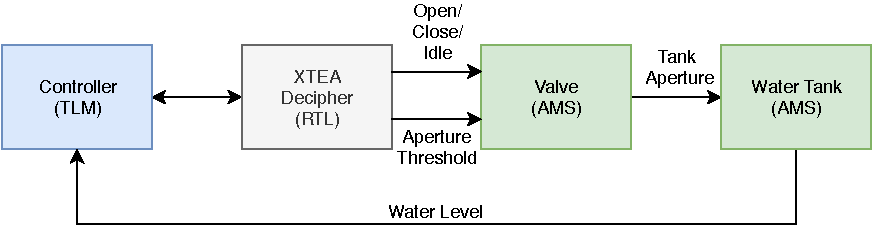
\includegraphics[width=\columnwidth]{figures/system.pdf}
	\caption{Organizzazione in moduli del sistema.}
	\label{fig:system}
\end{figure}

Il sistema descritto in questo documento deve monitorare e controllare il livello dell'acqua in un serbatoio. La figura 
\ref{fig:system} 
ne mostra la struttura, organizzata nei seguenti moduli:
\begin{itemize}
    \item Controller, si occupa di leggere il livello dell'acqua ricevuto dal serbatoio, e di inviare sulla base di 
    questo un comando ai moduli successivi, in modo da controllare l'apertura della valvola sulla base di un limite 
    massimo (anche questo calcolato e inviato dallo stesso controllore) per fare riempire il serbatoio. Da notare che 
    questo modulo cifra tutte le informazioni prima di inviarle agli altri moduli.
    
    \item XTEA Decipher, si occupa di decifrare i messaggi ricevuti dal Controller secondo l'agoritmo eXtended TEA 
    (interessante in questo caso poich\'e utilizza poche risorse hw, adattandosi perfettamente a questo tipo di sistema 
    embedded), per poi inviarli direttamente al modulo che aziona la valvola.
    
    \item Valve, applica i comandi che gli sono stati inviati dal Controller, modificando l'apertura/chiusura della 
    valvola per far riempire il serbatoio.
    
    \item Water Tank, \`e il sistema dinamico che si occupa del controllo dell'acqua sulla base della seguente funzione:
     \[\dot{x} = 0.6 * a - 0.03 * x\]
     dove $a$ \`e l'apertura della valvola e $x$ \`e il livello dell'acqua.
\end{itemize}

Nell'introduzione viene descritto in maniera astratta quello che poi viene dettagliato nel seguito del report. Una buona 
scaletta per l'introduzione pu\`o essere la seguente:
\begin{itemize}
\item Descrizione ad alto livello delle principali caratteristiche del sistema che si vuole modellare.
\item Descrizione delle motivazioni principali per l'utilizzo delle tecnologie descritte nel corso. Qual'\`e il problema 
che si vuole risolvere?
\item Descrizione dei passi utilizzati per arrivare all'implementazione finale. Descrivere la motivazione di ciascun 
passo. La descrizione dei passi dovrebbe 
formare la descrizione del flusso di lavoro svolto per completare l'assignment.
\item Rapidissima descrizione dei risultati principali.
\end{itemize}

L'introduzione non dovrebbe andare oltre la met\`a della seconda colonna (nel caso a due colonne), o la prima pagina 
(nel caso a colonna singola): bisogna cercare di essere concisi (e chiari). Alla fine, l'introduzione \`e solo 
``chiacchiere'': deve semplicemente rendere chiari quali sono gli obiettivi del lavoro (\emph{e nel caso del corso, deve 
far capire a me che avete gli obiettivi chiari in testa}). Consiglio: l'introduzione (e spesso l'abstract) \`e l'ultima 
parte che viene completata.

\section{Background}
Il sistema \`e stato implementato interamente in C++, utilizzando la libreria SystemC, poich\'e una delle motivazioni 
principali all'utilizzo di questa libreria \`e quello di poter integrare e simulare i vari componenti assieme, sviluppati 
a diversi livelli di astrazione. In particolare, i livelli di astrazione utilizzati sono:
\begin{itemize}
    \item SystemC RTL\cite{RTL} (Register Transfer Level), per una modellazione a basso livello, e dunque pi\`u vicina 
    all'hardware, con sviluppo dei moduli suddividendo la parte di logica di controllo, (\textit{fsm}), dalla parte che 
    esegue i calcoli e le operazioni aritmetiche/logiche (\textit{datapath}).
    
    \item SystemC\cite{SystemC} TLM (Transaction-level Modeling), che permette di descrivere come i vari moduli 
    interagiscono tra loro, grazie ai diversi stili messi a disposizione dalla libreria, ovvero TLM AT (approximately-
    timed) e TLM LT (loosely-timed) per una sincronizzazione basata su chiamate non bloccanti e/o basata sul concetto 
    del temporal decoupling rispettivamente, per arrivare ad una sincronizzazione a chiamate bloccanti in cui non si 
    tiene traccia del tempo di simulazione, e dunque molto pi\`u vicina ad una descrizione algoritmica, coincidente con 
    lo stile TLM UT (untimed).
    
    \item SystemC AMS\cite{AMS} (Analog/Mixed-Signal), che permette di modellare componenti analogiche e/o mixed-signal 
    utilizzando diversi tipi di formalismi quali TDF (Timed Data Flow) per una modellazione non conservativa di sistemi 
    a tempo discreto, LSF (Linear Signal FLow) per una modellazione non conservativa di sistemi a tempo discreto e a 
    tempo continuo (utilizzando solver automatici per risolvere le equazioni differenziali o alle differenze che 
    descrivono il sistema), e ELN (Electrical Linear Network) per una modellazione conservativa di sistemi a tempo 
    continuo.
\end{itemize}

\section{Metodologia applicata}

Le specifiche del progetto richiedevano di strutturare il sistema in moduli che possano essere implementati secondo i 
diversi livelli di astrazione messi a disposizione dalla libreria SystemC. Di seguito verranno illustrate nel dettaglio 
le caratteristiche di ciascun modulo:

\subsection{Xtea [RTL/TLM]}
Il modulo XTEA implementa l'agoritmo eXtended TEA, ideato da David Wheeler e Roger Needham al Cambridge Computer 
Laboratory. Il vantaggio principale di questo algoritmo \`e quello di avere una struttura semplice per poter essere 
impiegato in sistemi di limitate risorse hardware, e quindi il suo impiego si adatta perfettamente ad un sistema embedded
semplice quale quello che stiamo modellando, per poter offrire un minimo livello di sicurezza. A partire dai sorgenti i
n C/C++ \`e stato possibile ricavare la seguente struttura di base: 
\begin{figure}[h]
    \centering
    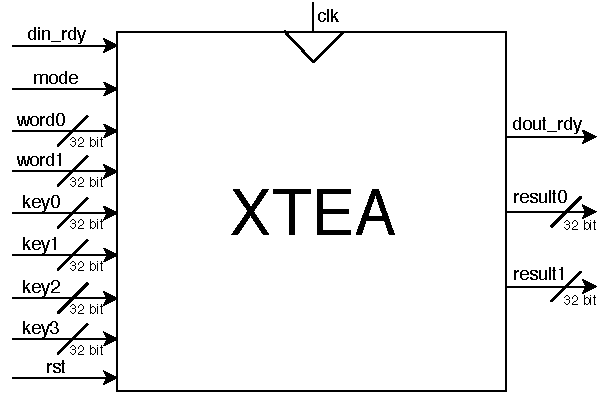
\includegraphics[width=0.7\columnwidth]{figures/xtea.pdf}
	\caption{Rappresentazione del modulo XTEA}
    \label{fig:xtea}
\end{figure}

Di seguito vengono descritti i diversi livelli di astrazione in cui il modulo \`e stato implementato:
\begin{itemize}
    \item XTEA RTL, descritto in SystemC RTL, \`e stato progettato suddividendo (secondo quanto detto precedentemente) 
    la parte di controllo dalla parte relativa ai calcoli. In figura~\ref{fig:fsmd} vengono presentate le porte di 
    ingresso e di uscita del modulo e i segnali che interconnettono l'FSM al Datapath. In particolare, l'FSM è sensibile
    alle variazioni sul segnale \state{din\_rdy} e \state{status}, mentre utilizza \state{mode} e \state{counter} per 
    decidere lo stato prossimo. Il Datapath invece è sensibile ai segnali di \state{reset} e \state{clock}, e utilizza 
    \state{mode}, \state{word\_0}, \state{word\_1} per calcolare i valori di output \state{result\_0} e \state{result\_1}. 
    Per quanto riguarda i segnali interni, nel datapath vengono definiti i seguenti:
    \begin{itemize}
        \item \state{k}, segnale a 2 bit per memorizzare quale delle 4 chiavi in input utilizzare nel calcolo;
        \item \state{key}, segnale a 32 bit per memorizzare temporaneamente la chiave da utilizzare;
        \item \state{delta}, per memorizzare il valore del parametro delta;
        \item \state{sum}, segnale a 64 bit utilizzato per i calcoli ad ogni iterazione;
        \item \state{counter}, segnale a 7 bit, utilizzato per le 64 iterazioni del ciclo per le due modalità (il motivo 
        per cui è stato scelto di effettuare 64 iterazioni invece di 32 verrà chiarito più avanti). Sono sufficienti 6 
        bit per compiere 64 iterazioni ma poiché all'ultima iterazione il segnale viene ulteriormente incrementato di 
        una unità, questo dev'essere a 7 bit per non perdere di informazione;
        \item \state{v0} e \state{v1}, segnali di appoggio per i calcoli, a 32 bit.
    \end{itemize}
    Nella descrizione del modulo secondo la EFSM\footnote{Extended Finite State Machine} in figura \ref{fig:efsm} (in 
    appendice), la parte di logica di controllo \`e rappresentata dalle transizioni e dalle condizioni sulle transizioni, 
    mentre il Datapath \`e rappresentato dagli stati dell'automa. A partire dagli stati \state{ST\_M0}, \state{ST\_K}, 
    \state{ST\_CALC} e \state{ST\_SUM} per la modalit\`a di cifratura (e equivalentemente \state{ST\_M1}, \state{ST\_K}, 
    \state{ST\_CALC} e \state{ST\_SUM} per la modalit\`a di decifratura) \`e possibile vedere come sia stato scelto, a 
    differenza della versione dell'algoritmo di C/C++, di effettuare un numero pari a 64 iterazioni per poter 
    riutilizzare i blocchi che altrimenti sarebbero ripetuti per le due modalit\`a. Inoltre, per quanto riguarda lo stato 
    \state{ST\_CALC} che tra tutti sembrerebbe essere quello a complessit\`a pi\`u alta, \`e stato scelto di non 
    spezzarlo in due stati in quanto le operazioni al suo interno risutano essere molto simili, e dunque un'eventuale 
    ottimizzazione dell'area secondo gli algoritmi allo stato dell'arte ne ridurrebbe drasticamente sia la complessit\`a, 
    sia gli elementi hardware da impiegare.
    
    \begin{figure}[bt]
        \centering
        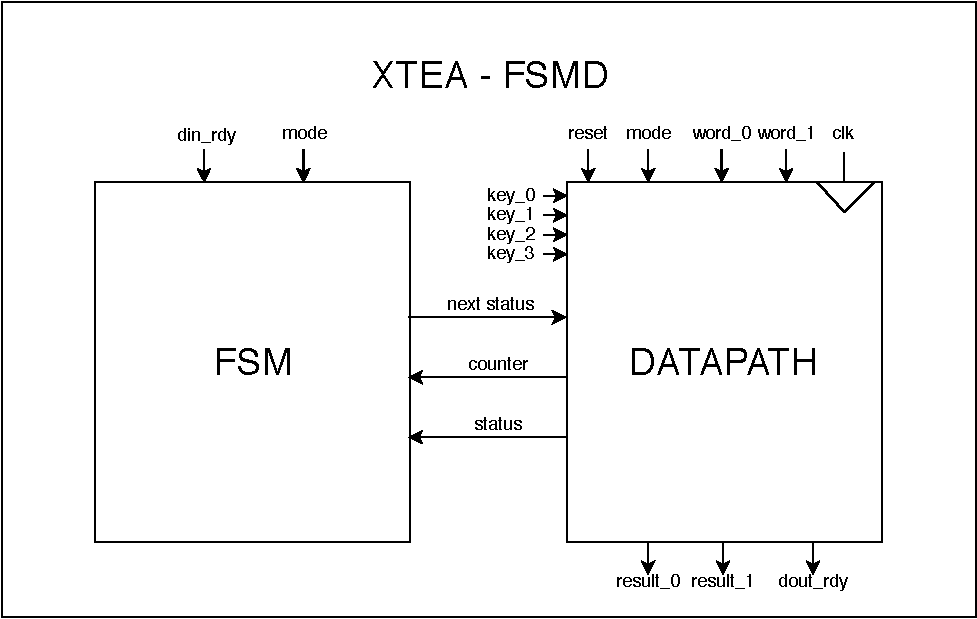
\includegraphics[width=0.9\columnwidth]{figures/fsmd.pdf}
        \caption{FSMD del modulo XTEA RTL}
        \label{fig:fsmd}
    \end{figure}

    \item XTEA TLM \`e la versione di XTEA sviluppata in SystemC TLM (nelle relative varianti UT, LT e AT4). La 
    struttura cha accomuna tutti e tre i moduli è la seguente: il \emph{testbench} (che implementa l'interfaccia 
    \code{tlm\_bw\_transport\_if}) effettua la funzionalit\`a dell'initiator, ovvero esegue le chiamate alla controparte 
    \emph{xtea} (che di conseguenza effettua la funzionalit\`a del target, implementando l'interfaccia 
    \code{tlm\_fw\_transport\_if}), avviando transazioni per permettere lo scambio di messaggi, che in questo caso, 
    corrispondono all'invio dei dati da cifrare/decifrare. In particolare, ad ogni transazione viene inviato un payload 
    esteso, ovvero un payload con allegate le informazioni definite nella struttura \code{iostruct}, che racchiude gli 
    input e gli output definiti nella rappresentazione in figura~\ref{fig:xtea}. 
    
    \begin{itemize}
        \item TLM Aproximately Timed (4 phases), è la versione basata su chiamate non bloccanti. La sincronizzazione 
        avviane secondo il classico protocollo di handshake a 4 fasi, in particolare il \emph{testbench} invia i dati 
        alla parte \emph{xtea} mettendosi successivamente in attesa dell'acknowledgement (fasi \code{BEGIN\_REQ}, 
        \code{END\_REQ}), \emph{xtea} riceve la transazione, elabora i dati e ne salva il risultato, per poi successivamente 
        ritornare l'acknowledgement alla controparte sbloccandone l'esecuzione (fasi \code{BEGIN\_RESP}, 
        \code{END\_RESP}).
        \item Loosely Timed, \`e la versione basata su una sincronizzazione a chiamate bloccanti. Qui l'initiator (che, 
        come detto sopra, è il \emph{testbench}) chiama la funzione \code{b\_transport} implementata nel target, 
        aggiungendo alla transazione, oltre al payload per lo scambio dei messaggi, anche l'informazione relativa al 
        tempo. Questa viene utilizzata per sfruttare il cosidetto Temporal Decoupling, ovvero per permettere ai processi 
        (nel nostro caso il testbench) di continuare la propria esecuzione senza per\`o incrementare il tempo di 
        simulazione, per poi sincronizzarsi esplicitamente in punti definiti oppure allo scadere del quanto di tempo 
        che gli è stato associato dallo scheduler, riducendone cos\`i il tempo totale della simulazione.
        \item TLM Untimed \`e una versione simile alla precedente, in cui non viene per\`o specificata l'informazione 
        relativa al tempo. Non richiede dunque una sincronizzazione esplicita, poich\`e questa viene garantita dalla 
        chiamata bloccante alla \code{b\_transport}, permettendo una classica sincronizzazione dei processi.
    \end{itemize}
\end{itemize}
La differenza tra queste quattro versioni sta nel tempo di simulazione. In tabella \ref{tab:time} vengono presentate le 
statistiche di simulazione basate su un'esecuzione di 1000 iterazioni per modulo, le quali mettono in evidenza come la 
versione RTL richieda più tempo di simulazione rispetto alle altre, poich\`e \`e la versione di XTEA pi\`u precisa, 
ovvero quella che garantisce una sincronizzazione tra le parti pi\`u accurata. Gli altri moduli (TLM), essendo meno 
accurati in termini di sincronizzazione, impiegano meno tempo di simulazione, con una differenza che cala gradualmente 
con l'aumento del livello di astrazione.
\begin{table}[]
    \centering
    \begin{tabular}{lllll}
    \toprule
                & UT     & LT     & AT4    & RTL    \\ \hline
    Real time   & 0,039s & 0,045s & 0,069s & 1,025s \\
    User time   & 0,009s & 0,015s & 0,016s & 0,894s \\
    System time & 0,018s & 0,018s & 0,044s & 0,052s \\ \bottomrule
    \\
    \end{tabular}
    \caption{Statistiche di esecuzione di XTEA secondo i diversi livelli di astrazione}
    \label{tab:time}
\end{table}

\subsection{Wwatertank System [AMS]}

Water Tank System è un sistema per il controllo e il monitoraggio del livello dell'acqua di un serbatoio. La modellazione,
che segue la struttura presentata in figura \ref{fig:continuous_system}, ha richiesto l'utilizzo di SystemC AMS, poich\'e 
i componenti da modellare presentano tutti comportamenti a tempo discreto e/o a tempo continuo.
\begin{figure}[bt]
	\centering
	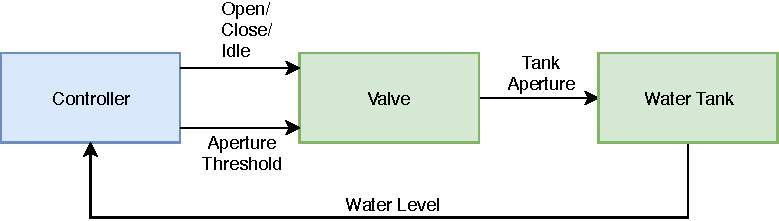
\includegraphics[width=\columnwidth]{figures/countinous_system.pdf}
	\caption{Struttura del watertank system}
	\label{fig:continuous_system}
\end{figure}
In particolare, il Controller, descritto in SystemC AMS utilizzando il formalismo TDF per una modellazione a tempo discreto, 
deve leggere il livello dell'acqua fornitogli in input e deve poi verificare che stia dentro il range $[5 \dots 8.8]$. 
Inoltre, sulla base delle condizioni riportate in tabella \ref{tab:behaviour}, il modulo deve periodicamente inviare al 
suo immediato vicino un comando di apertura o chiusura della valvola per fare riempire il serbatoio, e una threshold per 
indicare il livello di apertura massima che la valvola deve raggiungere. Dell'attuazione del comando si occuper\`a il 
modulo Valve, descritto anche questo secondo il formalismo TDF non conservativo per una modellazione a tempo discreto, 
mentre il modulo Water Tank è il componente che rileva il livello dell'acqua. Il suo comportamento rispecchia il seguente 
modello matematico, rappresentato sotto forma di schema a blocchi, e dunque si è scelto di descriverlo utilizzando 
il formalismo LSF non conservativo a tempo continuo, che aiuta nella risoluzione dell'equazione differenziale associata 
al modello grazie ai solver automatici che la libreria mette a disposizione:\\

\begin{table}[]
    \centering
    \begin{tabular}{lll}
    \toprule
    Water level     & Command   & Aperture threshold\\ \hline
    $range(5,8.8)$  & IDLE      & - \\
    $>8.8$          & CLOSE     & $t = t * 0.7$\\
    $<5$            & OPEN      & $t = t * 1.1$\\ \bottomrule
    \\
    \end{tabular}
    \caption{Parametri che influenzano il controllo sulla valvola}
    \label{tab:behaviour}
\end{table}  

\tikzstyle{block} = [draw, rectangle, minimum height=3em, minimum width=5em]
\tikzstyle{sum} = [draw, circle, node distance=1cm]
\tikzstyle{input} = [coordinate]
\tikzstyle{output} = [coordinate]

\resizebox{0.95\columnwidth}{!}{%
\begin{tikzpicture}[auto, node distance=1.5cm,>=latex']
    \node [input, name=input] {};
    \node [block, right of=input] (k1) {0.6};
    \node [sum, right of=k1, node distance=2.3cm] (sum) {};
    \node [block, right of=sum, node distance=1.8cm] (integral) {$\int$};
    \coordinate [right of=integral] (tmp);
    \node [block, below of=integral, node distance=1.5cm] (k2) {0.03};
    \node [output, right of=tmp] (output) {};
    \coordinate [below of=tmp] (tmp1);
    \coordinate [below of=sum] (tmp2);

    \draw [draw,->] (input) -- node {$a$} (k1);
    \draw [->] (k1) -- node {$sig_1$} (sum);
    \draw [->] (sum) -- node {$x'$} (integral);
    \draw [->] (integral) -- node {} (tmp) -- node [name=y] {$x$}(output);;
    \draw [->] (tmp) |- (tmp1) |- node {} (k2);
    \draw [->] (k2) -| (tmp2) -| node {$sig_2$} (sum);
\end{tikzpicture}
}
Ai capi di questo modello sono stati posizionati (in input e in output) dei convertitori da TDF a LSF e da LSF a TDF per
potersi interfacciare con gli altri moduli (descritti in SystemC AMS-TDF appunto) a tempo discreto.
Inoltre, per evitare problemi dovuti al loop creato, \`e stato inserito un delay sulla porta water\_level del Controller.

Per quanto riguarda la stabilizzazione dell'acqua, questa, come mostrato in figura \ref{fig:water_continuous_system}, 
si stabilizza approsimativamente attorno ai 200 secondi.
\begin{figure}[bt]
	\centering
	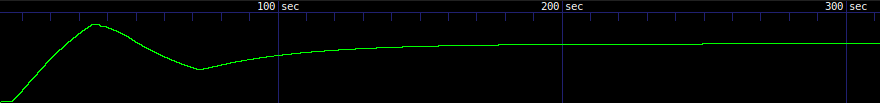
\includegraphics[width=0.95\columnwidth]{figures/water_level_continuous_subsystem.png}
	\caption{Stabilizzazione dell'acqua relativamente al Water Tank System (AMS) - Continous Subsystem}
	\label{fig:water_continuous_system}
\end{figure}

\subsection{Heterogeneous Platform}

L'Heterogeneous platform, ovvero l'unione in un unico sistema di tutti i moduli (descritti ognuno secondo un proprio
livello di astrazione) visti fin'ora e gi\`a presentato in parte nella sezione \ref{sec:intro}, \`e caratterizzato, 
oltre che da questi moduli appunto, anche da ulteriori 4 componenti, necessari per poter simulare l'intero sistema: i transattori. 
Nella figura \ref{fig:heterogeneous} \`e possibile vedere come questi componenti trasformano un segnale di interconnessione:
\begin{itemize}
    \item da TLM a RTL, per i segnali che partono dal Controller (in TLM) e che vengono inviati al modulo Xtea Decipher 
    (in RTL);
    \item da RTL a AMS, per i segnali che partono dal modulo Xtea Decipher e che entrano nel modulo Valve (in AMS);
    \item da AMS a RTL e nuovamente a TLM, per i segnali in uscita dal modulo Tank (in AMS) ed entranti nel modulo 
    Controller (TLM);
\end{itemize}
Da notare che i componenti Valve Interface e Tank Interface mostrati in figura, sono interfacce RTL necessarie per poter 
far comunicare tra loro moduli scritti in TLM, con moduli scritti in AMS e viceversa. Il modulo Valve Interface inoltre,
contiene al suo interno una parte di logica per riconoscere quando il modulo Xtea Decipher gli manda un comando oppure
una threshold. Queste informazioni infatti, sono inviate in due momenti separati e servono per utilizzare lo stesso 
componente per decifrare due tipologie di informazione diverse che gli vengono passate dal Controller (tramite l'Xtea
Transactor).


\section{Risultati}

Qua vanno ``messi i numeri''. Questa sezione dovrebbe contenere i risultati della simulazione. La simulazione mostra che 
il sistema funziona correttamente? Come \`e stato provato? Che tipo di testbench sono stati utilizzati? Come \`e stato 
scomposto il sistema per verificarne la correttezza?

Per quanto riguarda le performance:
\begin{itemize}
\item cosa si pu\`o dire in merito ai tempi di simulazione dei modelli a diversi livelli di astrazione? Quali dati 
supportano questa affermazione? Come sono stati ottenuti i dati?
\item Come cambia la velocit\`a di simulazione per la parte digitale e la parte a tempo continuo? Come influiscono le 
frequenze scelte? E i livelli di astrazione? \emph{etc.}
\end{itemize}

Questa sezione pu\`o contenere anche riflessioni personali sui risultati ottenuti. Importante: tutte le affermazioni 
devono essere supportate da numeri\footnote{Richard Feynman on Scientific Method (1964) -\\ 
https://www.youtube.com/watch?v=OL6-x0modwY}.

\section{Conclusioni}
Le conclusioni dovrebbero riassumere in poche righe  tutto ci\`o che \`e stato fatto. Un paio di righe descrivono i 
risultati osservati, in modo da introdurre poi la conclusione ``vera e propria''. Nel caso del corso, la ``lezione da 
portare a casa'' sar\`a quello che si \`e imparato svolgendo l'elaborato.


\bibliographystyle{IEEEtran}
\bibliography{biblio}

\appendix
\begin{figure*}[bt]
	\centering
	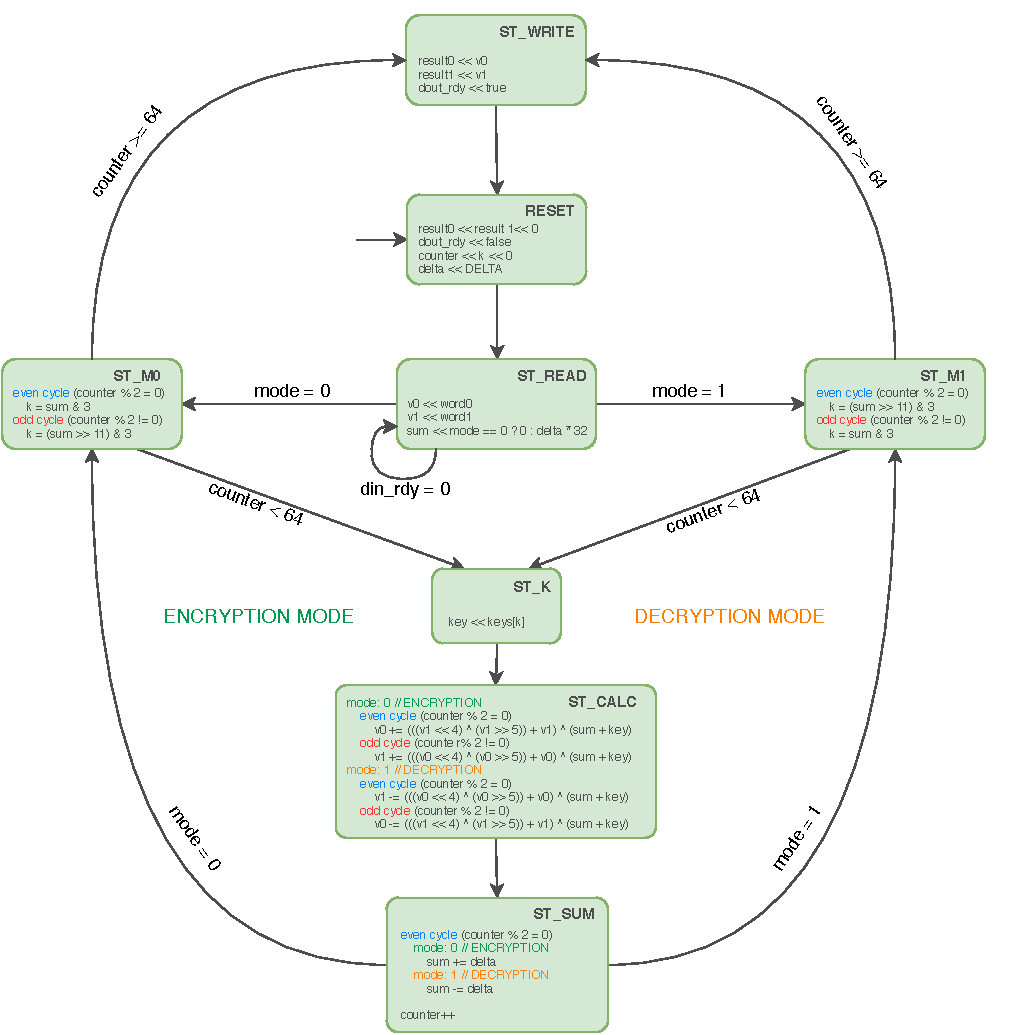
\includegraphics[width=0.7\textwidth]{figures/efsm.pdf}
	\caption{EFSM del modulo XTEA RTL}
	\label{fig:efsm}
\end{figure*}
\begin{figure*}[bt]
	\centering
	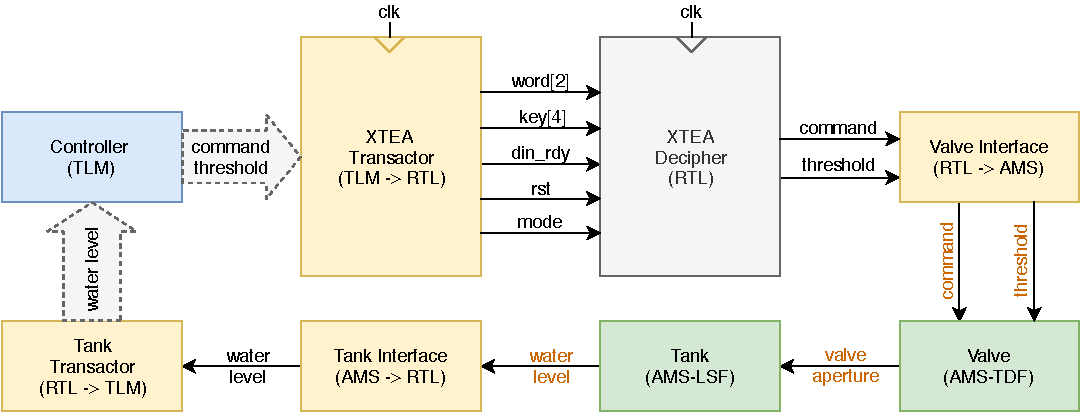
\includegraphics[width=0.7\textwidth]{figures/heterogeneous.pdf}
	\caption{Struttura del heterogeneous platform}
	\label{fig:heterogeneous}
\end{figure*}

Se non avete abbastanza spazio, potete inserire le figure delle EFSM in una  pagina extra, appendice. Un esempio di come 
potete fare solo le Figure~\ref{fig:grande}, \ref{fig:piccola1}, \ref{fig:piccola2}.

\end{document}